\subsection{2D Validation}
\label{sec:pyproct_supp_6}

In order to improve the reliability of pyProCT we have performed two
different quality assurance methods. The first was to ensure that
the software itself was working correctly using a unit testing methodology
(trying to get the best possible test coverage). The second was centered
in the validation of the clustering algorithms and the protocol.

Clusterings are hard to validate, especially when using
multidimensional data. Validating a 2D clustering, however, can be
an easier task as it can be visually checked. To this end we coded
the scripts that can be found in the folder\texttt{ pyproct/validation/bidimensional/}.


\subsubsection{Datasets}

To perform the validation, we downloaded some of Helmuth Spaeth's\cite{spaeth_spaeth_????-1}
datasets. These datasets have different characteristics that make them
difficult to cluster : 
\begin{enumerate}
	\item In this dataset 3 to 5 clusters can be seen. It looks like some of
	them can be subdivided. In general, these clusters are compact.
	\item It shows a set of points homogeneously covering the plane. There is not noticeable
	density variations.
	\item In this case there are two different density regions. In the bottom-right
	corner there is a compact cluster. The remaining points are sparsely
	distributed in the remaining space .
	\item Two compact clusters to the left, one big cluster (which seems to
	be composed of other clusters) sits on the right.
	\item Three parallel elongated clusters of different sizes and densities.
	\item Three elongated clusters with similar densities sharing the same origin.
	\item Two overlapped elongated clusters with different densities.
	\item Three elongate clusters with similar densities. All three are overlapped.
\end{enumerate}

We also used a code adapted from Jochen Wersdrfer's blog \cite{wersdorfer_spectral_????}
to generate a 9th dataset, which contains 450 points lying in three
concentric circles.


\subsubsection{Protocol validation}

In the first version of the validation script we used the datasets
to validate the algorithms, that is, we coded some algorithm-parameter
pairs and checked a picture of the resulting clusterings. Since the
algorithms were working as expected, we upgraded the script to fully
test the HCE protocol.

For each dataset, two hypotheses about the noise, cluster size and
number of clusters were defined (see \ref{tab:description_table})
based on our observations of the datasets. Also, we used two different
criteria to describe the expected clusterings:

\begin{description}
	\item [``default\_criteria''] Uses Silhouette and Cohesion ICVs. Is
	the default criteria of pyProCT and fosters both separation and compactness.
	\item [``graph\_criteria''] Uses the 'NCut' ICV. It tries to separate
	a graph representation of the dataset into connected components so
	that the sum of inner edge weights is optimized.
\end{description}

\begin{figure}
	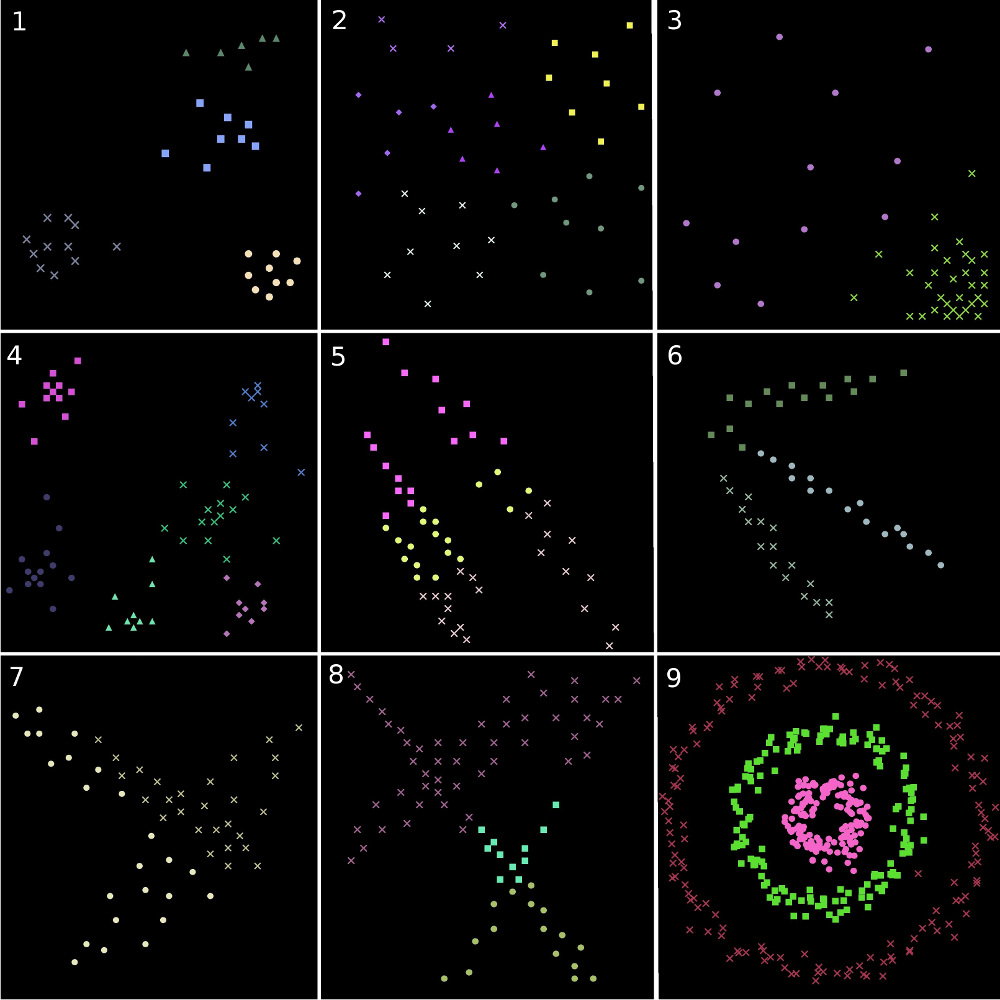
\includegraphics[width=\textwidth,height=\textheight,keepaspectratio]{pyproct_supp_c_plots}

	\protect\caption{Results of the application of pyProCT to nine 2D datasets. Clusters
	are plotted using different colors and symbols.\label{fig:plots_2d}}

\end{figure}

\begin{table}
\centering
\begin{tabular}{ c c c c c c }
\toprule
Dataset & \specialcell{Min.\\Clusters} & \specialcell{Max.\\Clusters} & \specialcell{Min.\\Cluster Size} & \specialcell{Max.\\Noise} & Criteria\\
\midrule
1 & 2 & 10 & 3 & 10\% & ``default\_criteria''\\
2 & 2 & 10 & 2 & 10\% & ``default\_criteria''\\
3 & 2 & 10 & 10 & 10\% & ``default\_criteria''\\
4 & 2 & 10 & 8 & 10\% & ``default\_criteria''\\
5 & 3 & 10 & 10 & 5\% & \specialcell{``default\_criteria'' \\ and ``graph\_criteria''}\\
6 & 3 & 10 & 13 & 10\% & ``graph\_criteria''\\
7 & 2 & 10 & 10 & 10\% & \specialcell{``default\_criteria'' \\ and ``graph\_criteria''}\\
8 & 3 & 8 & 5 & 10\% & \specialcell{``default\_criteria'' \\ and ``graph\_criteria''}\\
9 & 3 & 4 & 100 & 5\% & ``graph\_criteria''\\
\bottomrule
\end{tabular} \protect\caption{Clustering hypothesis for each of the datasets.\label{tab:description_table}}


\end{table}

\begin{figure}
	\fittopageimage{pyproct_supp_concentric_circles}

	\protect\caption{An incorrect choice of the ICVs to express the desired resulting clustering
	traits can drastically modify the results. In this case the criteria
	was changed from ``graph\_criteria'' to ``default\_criteria'',
	favoring one of the clusterings generated by the K-Medoids algorithm.
	\label{fig:concentric_circles}}
\end{figure}


\subsubsection{Results}

Clusterings 1, 3, 4, 6 and 9 are in full accordance with
our expectations (see table \ref{tab:results_table} and Fig. \ref{fig:plots_2d}).
We thought that the optimum solution for dataset 2 could be to use
one single cluster encompassing all elements. However the final partition
in 5 clusters looks reasonable. 

Clustering 5, 7 and 8 are different of what our intuition dictates.
The main problem that pyProCT has when dealing with a dataset like
7 or 8 is that their ``natural'' clusters overlap i.e. there are
elements that belong to more than one cluster at the same time. This
could be overcome by adding fuzzy algorithms to the algorithms pool.
Despite this, results would look counterintuitive in any case, as its usefulness
in most scenarios implies to discretize the membership values.

Clustering 5 highlights a weakness of the HCE methodology: its success
depends on the ability of the user to convey their goals in the clustering
hypothesis. If the user is not able to express it using pyProCT built-in
ICVs (see Fig. \ref{fig:concentric_circles}) or the needed ICVs to define
the hypothesis are not yet implemented, it would be impossible for
users to get the best-fitted result for their problems. It is clear
that, in this case, none of the used criteria suffices to choose the
type of result we would like to obtain.

\begin{table}
\centering
\begin{tabular}{ c c c c c }
\toprule
Dataset & Algorithm & Num. Clusters & Noise & Criteria\\
\midrule
1 & Gromos & 4 & 8.10\% & ``default\_criteria''\\
2 & Spectral Clust. & 5 & 0\% & ``default\_criteria''\\
3 & K-Medoids & 2 & 0\% & ``default\_criteria''\\
4 & K-Medoids & 6 & 9.59\% & ``default\_criteria''\\
5 & K-Medoids & 3 & 0\% & ``graph\_criteria''\\
6 & DBSCAN & 3 & 4\% & ``graph\_criteria''\\
7 & K-Medoids & 2 & 0\% & ``graph\_criteria''\\
8 & K-Medoids & 3 & 5.19\% & ``graph\_criteria''\\
9 & Spectral Clust. & 3 & 0\% & ``graph\_criteria''\\
\bottomrule
\end{tabular}

\protect\caption{Details of the results. Last column indicates the criteria
that obtained the best score. \label{tab:results_table}}
\end{table}
